\documentclass{article}
\usepackage{tikz}
\usepackage{amsmath, amssymb}
\usetikzlibrary{matrix, backgrounds, fit, calc, positioning}

\begin{document}
	
	\begin{figure}[htbp]
		\centering
		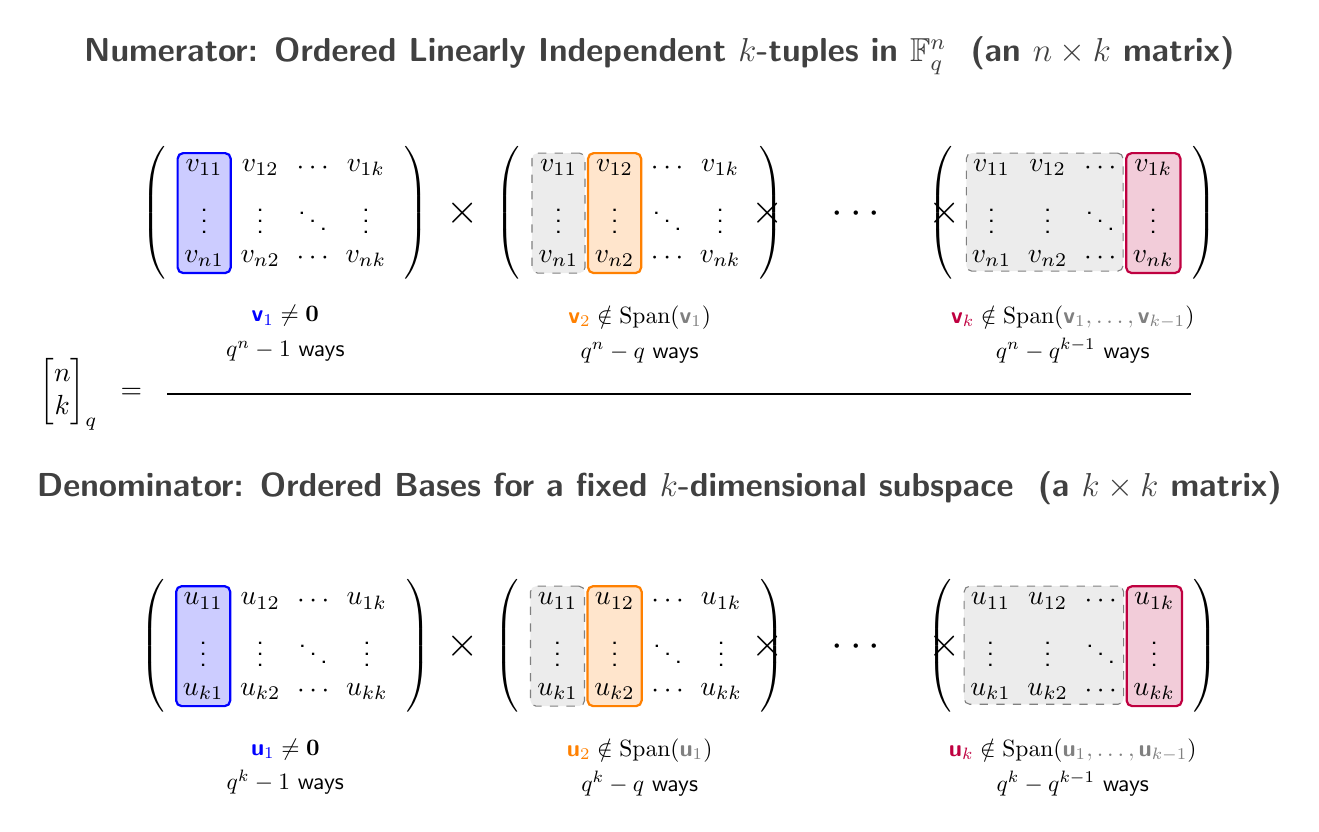
\begin{tikzpicture}[
			font=\sffamily,
			% Style for the matrices
			mtx/.style={
				matrix of math nodes,
				left delimiter=(, right delimiter=),
				nodes={minimum width=1.5em, inner sep=2pt, anchor=center},
				column sep=2pt, row sep=2pt,
				ampersand replacement=\&
			},
			% Highlighting styles for active columns
			hl-v1/.style={fill=blue!20, draw=blue, thick, rounded corners=2pt, inner sep=.25pt},
			hl-v2/.style={fill=orange!20, draw=orange, thick, rounded corners=2pt, inner sep=.25pt},
			hl-v4/.style={fill=purple!20, draw=purple, thick, rounded corners=2pt, inner sep=.25pt},
			% Style for the accumulating "Span Box"
			hl-span/.style={fill=gray!15, draw=gray, dashed, rounded corners=2pt, inner sep=.25pt},
			% Title & Text
			mainTitle/.style={font=\sffamily\bfseries\large, color=darkgray, align=center},
			term label/.style={font=\bfseries\small, align=center}
			]
			
			% ==============================================================================
			% NUMERATOR: Ordered Linearly Independent k-tuples in F_q^n
			% ==============================================================================
			\node[mainTitle] at (4.75, 4.5) {Numerator: Ordered Linearly Independent $k$-tuples in $\mathbb{F}_q^n$ \ (an $n \times k$ matrix)};
			
			% Matrix N1 (Column 1)
			\matrix[mtx] (N1) at (0, 2.5) {
				v_{11} \& v_{12} \& \cdots \& v_{1k} \\
				\vdots \& \vdots \& \ddots \& \vdots \\
				v_{n1} \& v_{n2} \& \cdots \& v_{nk} \\
			};
			\begin{scope}[on background layer] \node[hl-v1, fit=(N1-1-1)(N1-3-1)] {}; \end{scope}
			\node[below=0.2cm of N1, align=center, scale=0.85] {
				$\textcolor{blue}{\textbf{v}_1} \neq \mathbf{0}$ \\[1mm]
				\textbf{$q^n - 1$} ways
			};
			
			% Multiply Sign
			\node[scale=1.5] at (2.25, 2.5) {$\times$};
			
			% Matrix N2 (Column 2)
			\matrix[mtx] (N2) at (4.5, 2.5) {
				v_{11} \& v_{12} \& \cdots \& v_{1k} \\
				\vdots \& \vdots \& \ddots \& \vdots \\
				v_{n1} \& v_{n2} \& \cdots \& v_{nk} \\
			};
			\begin{scope}[on background layer]
				\node[hl-span, fit=(N2-1-1)(N2-3-1)] {}; % v1 forbidden
				\node[hl-v2, fit=(N2-1-2)(N2-3-2)] {};
			\end{scope}
			\node[below=0.2cm of N2, align=center, scale=0.85] {
				$\textcolor{orange}{\textbf{v}_2} \notin \mathrm{Span}(\textcolor{gray}{\textbf{v}_1})$ \\[1mm]
				\textbf{$q^n - q$} ways
			};
			
			% Multiply Sign (Dots)
			\node[scale=1.5] at (7.25, 2.5) {$\times \quad \cdots \quad \times$};
			
			% Matrix Nk (Column k)
			\matrix[mtx] (Nk) at (10, 2.5) {
				v_{11} \& v_{12} \& \cdots \& v_{1k} \\
				\vdots \& \vdots \& \ddots \& \vdots \\
				v_{n1} \& v_{n2} \& \cdots \& v_{nk} \\
			};
			\begin{scope}[on background layer]
				\node[hl-span, fit=(Nk-1-1)(Nk-3-3)] {}; % v1 to v_{k-1} forbidden
				\node[hl-v4, fit=(Nk-1-4)(Nk-3-4)] {};
			\end{scope}
			\node[below=0.2cm of Nk, align=center, scale=0.85] {
				$\textcolor{purple}{\textbf{v}_k} \notin \mathrm{Span}(\textcolor{gray}{\textbf{v}_1, \dots, \textbf{v}_{k-1}})$ \\[1mm]
				\textbf{$q^n - q^{k-1}$} ways
			};
			
			% ==============================================================================
			% FRACTION LINE AND RESULT
			% ==============================================================================
			\draw[thick] (-1.5, 0.2) -- (11.5, 0.2);
			\node[left] at (-1.5, 0.2) {$\displaystyle \begin{bmatrix} n \\ k \end{bmatrix}_q \;\; = \;\;$};
			
			% ==============================================================================
			% DENOMINATOR: Ordered Bases for a fixed k-dimensional subspace
			% ==============================================================================
			\node[mainTitle] at (4.75, -1.0) {Denominator: Ordered Bases for a fixed $k$-dimensional subspace \ (a $k \times k$ matrix)};
			
			% Matrix D1 (Column 1)
			\matrix[mtx] (D1) at (0, -3.0) {
				u_{11} \& u_{12} \& \cdots \& u_{1k} \\
				\vdots \& \vdots \& \ddots \& \vdots \\
				u_{k1} \& u_{k2} \& \cdots \& u_{kk} \\
			};
			\begin{scope}[on background layer] \node[hl-v1, fit=(D1-1-1)(D1-3-1)] {}; \end{scope}
			\node[below=0.2cm of D1, align=center, scale=0.85] {
				$\textcolor{blue}{\textbf{u}_1} \neq \mathbf{0}$ \\[1mm]
				\textbf{$q^k - 1$} ways
			};
			
			% Multiply Sign
			\node[scale=1.5] at (2.25, -3.0) {$\times$};
			
			% Matrix D2 (Column 2)
			\matrix[mtx] (D2) at (4.5, -3.0) {
				u_{11} \& u_{12} \& \cdots \& u_{1k} \\
				\vdots \& \vdots \& \ddots \& \vdots \\
				u_{k1} \& u_{k2} \& \cdots \& u_{kk} \\
			};
			\begin{scope}[on background layer]
				\node[hl-span, fit=(D2-1-1)(D2-3-1)] {}; % u1 forbidden
				\node[hl-v2, fit=(D2-1-2)(D2-3-2)] {};
			\end{scope}
			\node[below=0.2cm of D2, align=center, scale=0.85] {
				$\textcolor{orange}{\textbf{u}_2} \notin \mathrm{Span}(\textcolor{gray}{\textbf{u}_1})$ \\[1mm]
				\textbf{$q^k - q$} ways
			};
			
			% Multiply Sign (Dots)
			\node[scale=1.5] at (7.25, -3.0) {$\times \quad \cdots \quad \times$};
			
			% Matrix Dk (Column k)
			\matrix[mtx] (Dk) at (10, -3.0) {
				u_{11} \& u_{12} \& \cdots \& u_{1k} \\
				\vdots \& \vdots \& \ddots \& \vdots \\
				u_{k1} \& u_{k2} \& \cdots \& u_{kk} \\
			};
			\begin{scope}[on background layer]
				\node[hl-span, fit=(Dk-1-1)(Dk-3-3)] {}; % u1 to u_{k-1} forbidden
				\node[hl-v4, fit=(Dk-1-4)(Dk-3-4)] {};
			\end{scope}
			\node[below=0.2cm of Dk, align=center, scale=0.85] {
				$\textcolor{purple}{\textbf{u}_k} \notin \mathrm{Span}(\textcolor{gray}{\textbf{u}_1, \dots, \textbf{u}_{k-1}})$ \\[1mm]
				\textbf{$q^k - q^{k-1}$} ways
			};
			
		\end{tikzpicture}
	\end{figure}
	
\end{document}